\documentclass[10pt,a4paper]{article}
\usepackage[utf8]{inputenc}
\usepackage[italian]{babel}
\usepackage{amsmath}
\usepackage{amsfonts}
\usepackage{amssymb}
\usepackage[left=1cm,right=1cm,top=1cm,bottom=1cm]{geometry}

\usepackage{blindtext}
\usepackage[T1]{fontenc}
\usepackage[utf8]{inputenc}
\usepackage{graphicx}

\usepackage{subcaption}

\usepackage{titlesec}
\setcounter{secnumdepth}{4}
\titleformat{\paragraph}
{\normalfont\normalsize\bfseries}{\theparagraph}{1em}{}
\titlespacing*{\paragraph}
{0pt}{3.25ex plus 1ex minus .2ex}{1.5ex plus .2ex}





\begin{document}
\section{Dal machine learning al deep learning}
Oggi l'intelligenza artificiale è un fiorente campo di ricerca, con l'obiettivo di risolvere una grande varietà di problemi, che per essere risolti attraverso la programmazione classica necessitano di una grande quantità di conoscenze a riguardo, spesso non disponibile. I Programmi basati sul paradigma dell'intelligenza artificiale si propongono di superare questi ostacoli acquisendo direttamente queste conoscenze dai dati grezzi, tale capacità è nota come machine learning.

\begin{figure}[h!]
  \centering
  \begin{subfigure}[b]{0.45\linewidth}
  	\centering
    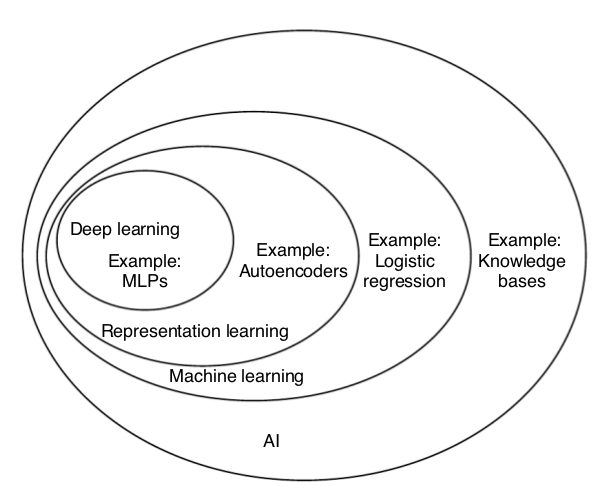
\includegraphics[height=200pt]{AI_venn_diagram.png}
    \caption{famiglie di algoritmi}
  \end{subfigure}
  \begin{subfigure}[b]{0.45\linewidth}
  	\centering
    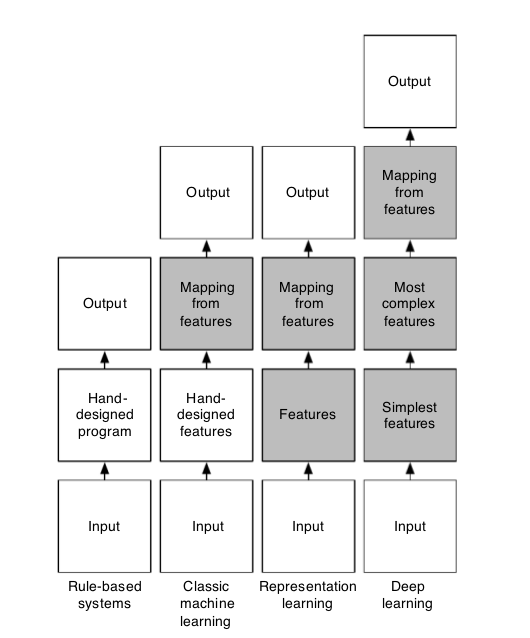
\includegraphics[height=200pt]{diff_between_aprochs.png}
    \caption{differenze tra le diverse tipologie}
  \end{subfigure}
  \label{fig:garph1}
\end{figure}

\end{document}